\documentclass[12pt,a4paper]{article}

\usepackage[utf8]{inputenc}
\usepackage[T1]{fontenc}
\usepackage{graphicx}
\usepackage{hyperref}
\usepackage{geometry}
\usepackage{booktabs}
\usepackage{float}
\usepackage{enumitem}
\usepackage{fancyhdr}
\usepackage{xcolor}
\usepackage{listings}
\usepackage{tikz}
\usepackage{colortbl}
\usepackage{mdframed}
\usepackage{fontawesome5}
\usepackage{setspace}

\geometry{margin=1in, headheight=15pt}
\onehalfspacing

\definecolor{primaryblue}{RGB}{26, 115, 232}
\definecolor{darkblue}{RGB}{13, 71, 161}
\definecolor{lightblue}{RGB}{232, 245, 253}
\definecolor{successgreen}{RGB}{46, 125, 50}
\definecolor{lightgray}{RGB}{248, 249, 250}

\hypersetup{colorlinks=true, linkcolor=darkblue, urlcolor=primaryblue}

\lstset{
    basicstyle=\ttfamily\small,
    breaklines=true,
    frame=single,
    backgroundcolor=\color{lightgray},
    rulecolor=\color{gray}
}

\newmdenv[
    linecolor=primaryblue,
    backgroundcolor=lightblue,
    linewidth=2pt,
    topline=false,
    rightline=false,
    bottomline=false,
]{highlightblock}

\newmdenv[
    linecolor=successgreen,
    backgroundcolor=successgreen!10,
    linewidth=2pt,
    topline=false,
    rightline=false,
    bottomline=false,
]{successblock}

\pagestyle{fancy}
\fancyhf{}
\fancyhead[L]{\small\color{gray}Individual Contribution Report}
\fancyhead[R]{\small\color{darkblue}\textbf{Aman Banajre}}
\fancyfoot[C]{\thepage}
\renewcommand{\headrulewidth}{0.5pt}
\renewcommand{\footrulewidth}{0.5pt}

\begin{document}

%========================================
% TITLE PAGE
%========================================
\begin{titlepage}
    \centering
    \vspace*{2cm}
    
    {\Large\color{gray} INDIVIDUAL CONTRIBUTION REPORT\\[0.3cm]}
    
    \rule{0.8\textwidth}{1pt}\\[0.5cm]
    
    {\Huge\bfseries\color{darkblue} Aman Banajre\\[0.5cm]}
    
    \rule{0.8\textwidth}{1pt}\\[1cm]
    
    {\Large\textit{Garbage Classifier for Waste Management}\\[0.3cm]}
    {\large AI-Powered Garbage Segmentation System\\[1.5cm]}
    
    \begin{tikzpicture}
        \node[draw=primaryblue, fill=lightblue, rounded corners=10pt, minimum width=8cm, minimum height=3cm, align=center] {
            \textbf{\large Primary Roles}\\[0.3cm]
            \faIcon{book} Documentation\\
            \faIcon{clipboard-check} Testing\\
            \faIcon{shield-alt} Quality Assurance
        };
    \end{tikzpicture}
    
    \vfill
    
    {\large
    \textbf{BTech (Hons.) CSE - Artificial Intelligence}\\
    5th Semester | Group 09\\[0.5cm]
    University Teaching Department (UTD)\\
    CSVTU, Bhilai\\[0.5cm]
    \textbf{December 2025}
    }
    
\end{titlepage}

\tableofcontents
\newpage

%========================================
% SECTION 1: ROLE OVERVIEW
%========================================
\section{Role Overview}

\begin{highlightblock}
\textbf{\faIcon{user-tag} Assigned Responsibilities:}
\begin{itemize}[leftmargin=*]
    \item[\faIcon{book}] \textbf{Documentation} — Technical and user documentation
    \item[\faIcon{clipboard-check}] \textbf{Testing} — Functional and UAT testing
    \item[\faIcon{shield-alt}] \textbf{Quality Assurance} — Code review and validation
\end{itemize}
\end{highlightblock}

%========================================
% SECTION 2: DOCUMENTATION
%========================================
\section{Documentation}

\subsection{User Documentation}

Created comprehensive user-facing documentation:

\begin{table}[H]
    \centering
    \caption{Documentation Components}
    \rowcolors{2}{lightgray}{white}
    \begin{tabular}{@{}lp{7cm}@{}}
        \toprule
        \rowcolor{darkblue}
        \textcolor{white}{\textbf{Document}} & \textcolor{white}{\textbf{Content}} \\
        \midrule
        Installation Guide & Step-by-step setup instructions \\
        Usage Guide & Interface walkthrough with examples \\
        API Reference & Function signatures and parameters \\
        Troubleshooting & Common issues and solutions \\
        \bottomrule
    \end{tabular}
\end{table}

\subsection{Usage Instructions}

\begin{table}[H]
    \centering
    \caption{Application Usage Guide}
    \rowcolors{2}{lightgray}{white}
    \begin{tabular}{@{}lp{7cm}@{}}
        \toprule
        \rowcolor{darkblue}
        \textcolor{white}{\textbf{Action}} & \textcolor{white}{\textbf{Description}} \\
        \midrule
        Upload Image & Click image area or drag-drop file \\
        Set Confidence & Adjust slider (0.1 to 0.95) \\
        Enable Enhancement & Toggle checkbox for better accuracy \\
        Detect & Click "Detect Garbage" button \\
        View Results & See annotated image and pie chart \\
        \bottomrule
    \end{tabular}
\end{table}

%========================================
% SECTION 3: TESTING
%========================================
\section{Testing}

\subsection{Functional Testing}

\begin{table}[H]
    \centering
    \caption{Functional Test Results}
    \rowcolors{2}{lightgray}{white}
    \begin{tabular}{@{}p{5cm}cc@{}}
        \toprule
        \rowcolor{darkblue}
        \textcolor{white}{\textbf{Test Scenario}} & \textcolor{white}{\textbf{Expected}} & \textcolor{white}{\textbf{Status}} \\
        \midrule
        Image upload works & Success & \textcolor{successgreen}{\faIcon{check}} \\
        Confidence slider functional & Updates detection & \textcolor{successgreen}{\faIcon{check}} \\
        Enhancement checkbox works & Toggles preprocessing & \textcolor{successgreen}{\faIcon{check}} \\
        Detect button triggers inference & Shows results & \textcolor{successgreen}{\faIcon{check}} \\
        Pie chart displays correctly & Correct distribution & \textcolor{successgreen}{\faIcon{check}} \\
        Summary text accurate & Matches detections & \textcolor{successgreen}{\faIcon{check}} \\
        \bottomrule
    \end{tabular}
\end{table}

\subsection{User Acceptance Testing}

Performed UAT with team members:
\begin{itemize}[leftmargin=*, label=\faIcon{users}]
    \item Tested with 5 team members
    \item Collected UI/UX feedback
    \item Identified usability improvements
    \item Verified output accuracy
\end{itemize}

\subsection{Edge Case Testing}

\begin{itemize}[leftmargin=*, label=\faIcon{exclamation-triangle}]
    \item Empty image upload
    \item Very large images (4K resolution)
    \item Images with no garbage
    \item Images with many objects (10+)
    \item Non-image file uploads
\end{itemize}

%========================================
% SECTION 4: QUALITY ASSURANCE
%========================================
\section{Quality Assurance}

\subsection{Quality Checklist}

\begin{table}[H]
    \centering
    \caption{QA Validation Checklist}
    \rowcolors{2}{lightgray}{white}
    \begin{tabular}{@{}lc@{}}
        \toprule
        \rowcolor{darkblue}
        \textcolor{white}{\textbf{Criterion}} & \textcolor{white}{\textbf{Status}} \\
        \midrule
        All functions documented & \textcolor{successgreen}{\faIcon{check-circle}} \\
        Error handling in place & \textcolor{successgreen}{\faIcon{check-circle}} \\
        Input validation complete & \textcolor{successgreen}{\faIcon{check-circle}} \\
        Output format consistent & \textcolor{successgreen}{\faIcon{check-circle}} \\
        Performance acceptable & \textcolor{successgreen}{\faIcon{check-circle}} \\
        UI responsive & \textcolor{successgreen}{\faIcon{check-circle}} \\
        Deployment successful & \textcolor{successgreen}{\faIcon{check-circle}} \\
        \bottomrule
    \end{tabular}
\end{table}

%========================================
% SECTION 5: ACHIEVEMENTS
%========================================
\section{Technical Achievements}

\begin{successblock}
\textbf{\faIcon{trophy} Key Accomplishments:}
\begin{itemize}[leftmargin=*, label=\faIcon{star}]
    \item Created comprehensive user documentation
    \item Conducted thorough functional testing
    \item Performed user acceptance testing
    \item Ensured code quality through reviews
    \item Validated deployment readiness
\end{itemize}
\end{successblock}

%========================================
% SECTION 6: SKILLS
%========================================
\section{Skills Demonstrated}

\begin{table}[H]
    \centering
    \rowcolors{2}{lightgray}{white}
    \begin{tabular}{@{}ll@{}}
        \toprule
        \rowcolor{darkblue}
        \textcolor{white}{\textbf{Category}} & \textcolor{white}{\textbf{Skills}} \\
        \midrule
        Documentation & Technical writing, user guides \\
        Testing & Functional, UAT, edge cases \\
        Quality & Code review, validation \\
        Communication & Clear documentation \\
        \bottomrule
    \end{tabular}
\end{table}

\end{document}
